%==============================================================================
%  MATH 231 -- Linear Algebra I (Queens College, Fall 2026)
%  VECTOR UNIT, PART 1 -- Vectors: Definition, Notation, and Arithmetic
%
%  This is one of three documents covering the vector unit. Section numbering
%  runs CONTINUOUSLY across all three, so that every cross-reference in the
%  unit means the same thing no matter which part it appears in:
%
%      Part 1  MATH231_vectors_1_definition_and_arithmetic  Sections 1-9
%      Part 2  MATH231_vectors_2_dot_product_and_projection Sections 10-12
%      Part 3  MATH231_vectors_3_norms_and_metrics          Sections 13-15
%
%  Parts 2 and 3 therefore begin with \setcounter{section}{...}.  Definitions
%  and examples are numbered BY SECTION (Definition 7.1, Example 11.2, ...) so
%  that they too are unique across the whole unit.
%
%  AUDIENCE: distributed to students.  Keep it free of instructor-facing
%  apparatus -- time budgets, pacing notes, teaching cues.
%
%  NOTATION ORDER: R^2 is introduced in Section 6 and must not appear before
%  it.  Sections 1-5 refer to "the plane" instead.  Section 6 also introduces
%  the signature notation f : A -> B, which Section 7 is the first to use.
%
%  OPERATION ARITY is a running thread: the norm (Sec. 2) is unary, addition
%  and subtraction (Sec. 7) are binary on two vectors, and scalar
%  multiplication (Sec. 8) is binary on a scalar and a vector.
%
%  ORDERING DEPENDENCY: the geometric reading of u - v as u + (-v) needs -v,
%  i.e. scalar multiplication by -1, so it lives in Sec. 8.3 and NOT in Sec. 7.
%  Sec. 7.3 gives the between-the-heads reading, which needs no scaling.
%  Equality of vectors (Sec. 9) is what licenses the head-to-tail picture in
%  Sec. 7.1; that debt is flagged forward where it is incurred.
%
%  Compile with pdflatex (standard TeX Live packages only; uses tikz).
%==============================================================================

\documentclass[11pt]{article}

\usepackage[margin=1in]{geometry}
\usepackage{amsmath,amssymb,amsthm}
\usepackage[dvipsnames]{xcolor}
\usepackage{enumitem}
\usepackage{booktabs}
\usepackage{array}
\usepackage[hidelinks]{hyperref}
\usepackage{titlesec}
\usepackage{needspace}
\usepackage{tikz}
\usetikzlibrary{arrows.meta}

%------------------------------------------------------------------ style ----
\titleformat{\section}{\large\bfseries\sffamily}{\thesection.}{0.6em}{}
\titleformat{\subsection}{\normalsize\bfseries\sffamily}{\thesubsection.}{0.5em}{}
\titlespacing*{\section}{0pt}{14pt}{6pt}

\theoremstyle{definition}
\newtheorem{defn}{Definition}[section]
\newtheorem{ex}{Example}[section]
\theoremstyle{remark}
\newtheorem*{rmk}{Remark}
\newtheorem*{warn}{A common confusion}

% Honest forward references: things we are simplifying on purpose today and
% will come back to later in the course.
\newcommand{\lookahead}{\par\smallskip\noindent
  \textbf{\sffamily\textcolor{RoyalBlue}{Looking ahead.}}\ \ignorespaces}

%--------------------------------------------------------------- notation ----
\newcommand{\R}{\mathbb{R}}
\newcommand{\vc}[1]{\mathbf{#1}}
\newcommand{\norm}[1]{\lVert #1\rVert}
\newcommand{\uv}[1]{\hat{\vc{#1}}}                 % normalized vector
\newcommand{\Sph}[1]{\mathbb{S}^{#1}}              % the #1-sphere
\newcommand{\proj}[2]{\operatorname{proj}_{#1}(#2)}
\newcommand{\comp}[2]{\operatorname{comp}_{#1}(#2)}

%------------------------------------------------------------- tikz helpers --
\tikzset{
  vecarr/.style   = {-{Stealth[length=2.6mm,width=2.0mm]},very thick},
  thinarr/.style  = {-{Stealth[length=2.2mm,width=1.7mm]},thick},
  axisline/.style = {->,gray!75,thin}
}
% \lattice{xmin}{xmax}{ymin}{ymax}
\newcommand{\lattice}[4]{%
  \draw[step=1cm,gray!25,very thin] (#1,#3) grid (#2,#4);
  \draw[axisline] (#1,0) -- (#2+0.45,0) node[right,font=\scriptsize,black]{$x$};
  \draw[axisline] (0,#3) -- (0,#4+0.45) node[above,font=\scriptsize,black]{$y$};
}
% bare axes, for the small orientation panels
\newcommand{\baxes}[4]{%
  \draw[axisline] (#1,0) -- (#2,0);
  \draw[axisline] (0,#3) -- (0,#4);
}


\title{\vspace{-1.2cm}\textbf{\sffamily MATH 231 -- Linear Algebra I}\\[4pt]
       {\large\sffamily The Vector Unit, Part 1 \textbullet\ Vectors:
        Definition, Notation, and Arithmetic}\\[2pt]
       {\normalsize\sffamily Kiely Hall 326 \textbullet\
        Instructor: Kevin Bedoya}}
\author{}
\date{}

\begin{document}
\maketitle
\vspace{-1.6cm}

\noindent\textbf{About this document.} The vector unit is split across three
parts, of which this is the first. Section numbering runs continuously through
all three, so a reference such as \S11.6 always points to the same place
regardless of which part you are reading:

\begin{center}
\renewcommand{\arraystretch}{1.2}
\begin{tabular}{@{}l l l@{}}
\toprule
\textbf{Part} & \textbf{Sections} & \textbf{Subject} \\
\midrule
1 & \S1--\S9   & vectors, notation, addition, scaling, equality \\
2 & \S10--\S12 & orientation, the dot product, projection \\
3 & \S13--\S15 & Cauchy--Schwarz, metrics, norms \\
\bottomrule
\end{tabular}
\end{center}

\noindent\textbf{What you should be able to do afterwards.} State what a vector
is in terms of magnitude and direction; identify the tail and head of a vector
in the plane; compute the Euclidean norm and explain why it is a \emph{unary}
operation; distinguish vector quantities from scalar quantities; read all three
notational conventions for a vector, and read a signature $f:A\to B$; add and
subtract vectors both componentwise and geometrically, using the parallelogram
rule and the triangle inequality; scale a vector by a real number and say what
$\alpha=-1$ does to it; and decide when two vectors drawn in different places
are the \emph{same} vector.

\medskip
\noindent\textbf{Further reading.}
Boyd \& Vandenberghe, \emph{Introduction to Applied Linear Algebra}, Ch.~1
(vectors, addition, scalar multiplication) and Ch.~3 (norm and distance);
Strang, \emph{Linear Algebra and Its Applications}, Ch.~1;
Axler, \emph{Linear Algebra Done Right}, Ch.~1.

%==============================================================================
\section{Vectors: magnitude, direction, and the space they live in}
%==============================================================================
We begin with a working definition --- deliberately informal, and stated in the
language of quantities rather than axioms.

\begin{defn}[Vector, working definition]
A \emph{vector} is a mathematical object carrying two attributes:
a \textbf{magnitude} and a \textbf{direction}.
\end{defn}

\lookahead This is the physicist's definition, and it is the right one to start
from because it is the one you can \emph{see}. Later in the course we replace it
with the algebraist's definition: a vector will become any element of a set
equipped with two operations obeying a short list of axioms --- at which point
functions, polynomials, and matrices all become vectors too, and ``magnitude and
direction'' stops being the defining feature. For now, hold on to the picture.

\subsection*{The space a vector lives in}
A vector does not exist in isolation; it lives in a space. Ours today is the
\textbf{two-dimensional Euclidean plane}, the familiar $xy$-plane, and every
vector we draw will live in it.

The word \emph{dimension} here means a \textbf{degree of freedom} with respect
to spatial coordinates: how many independent numbers must you supply to pin down
a location? On a line, one; on the plane, two --- an $x$ and a $y$, chosen
independently of one another. The plane is two-dimensional in exactly that
sense.

\subsection*{Tail, head, and the two attributes}
Fix the point $(1,2)$. Draw an arrow from the origin to it. That arrow is a
vector, and it has two distinguished points:

\begin{itemize}[leftmargin=1.4em,itemsep=2pt]
  \item the \textbf{tail} --- where the arrow begins, here the origin $(0,0)$;
  \item the \textbf{head} --- where the arrow ends and the arrowhead is drawn,
        here $(1,2)$.
\end{itemize}

\noindent With the tail and head named, the two attributes become concrete:

\begin{itemize}[leftmargin=1.4em,itemsep=2pt]
  \item \textbf{Direction} is the arrow's orientation in the plane --- which way
        it points, relative to the axes, as it travels from tail to head. The
        arrow to $(1,2)$ points up and to the right, more steeply up than
        rightward.
  \item \textbf{Magnitude} is the arrow's \textbf{length}: the distance from the
        tail to the head. We measure it with the Euclidean distance, and we
        compute it in \S2.
\end{itemize}

\noindent Note the arrowhead in the left-hand figure below: the arrowhead
\emph{is} the direction, so a bare line segment would lose half the
information.

\begin{center}
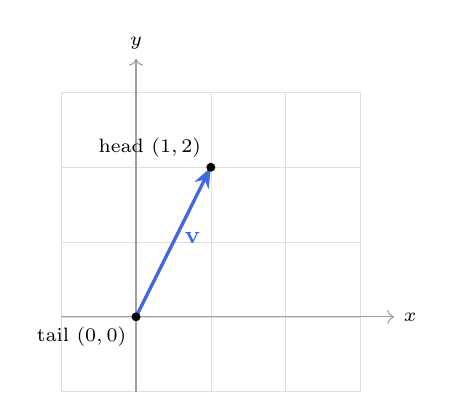
\begin{tikzpicture}[scale=0.95]
  \lattice{-1}{3}{-1}{3}
  \draw[vecarr,RoyalBlue] (0,0) -- (1,2);
  \fill (0,0) circle (1.7pt);
  \fill (1,2) circle (1.7pt);
  \node[below left,font=\scriptsize]  at (0,0) {tail $(0,0)$};
  \node[above left,font=\scriptsize]  at (1,2) {head $(1,2)$};
  \node[right,font=\small,RoyalBlue]  at (0.52,1.05) {$\vc{v}$};
\end{tikzpicture}
\hspace{1.4cm}
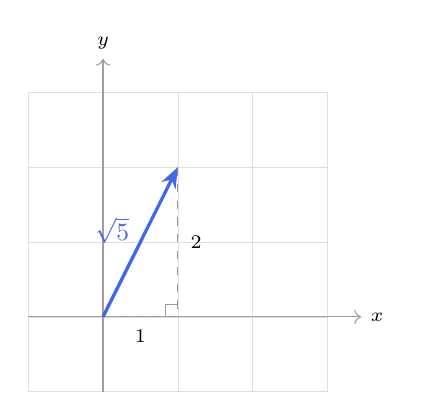
\begin{tikzpicture}[scale=0.95]
  \lattice{-1}{3}{-1}{3}
  \draw[dashed,gray!80] (0,0) -- (1,0) -- (1,2);
  \draw[gray!80] (0.84,0) -- (0.84,0.16) -- (1,0.16);
  \draw[vecarr,RoyalBlue] (0,0) -- (1,2);
  \node[below,font=\scriptsize] at (0.5,-0.04) {$1$};
  \node[right,font=\scriptsize] at (1.04,1) {$2$};
  \node[left,font=\small,RoyalBlue] at (0.48,1.15) {$\sqrt{5}$};
\end{tikzpicture}
\end{center}

%==============================================================================
\section{The norm --- our first vector operation}
%==============================================================================
The magnitude of a vector is not just a description of it; it is something we
\emph{compute} from it. Computing it is our first vector operation, and it has a
name.

\begin{defn}[Euclidean norm]
For a vector $\vc{v}$ in the plane with tail at the origin and head at $(x,y)$,
the \textbf{Euclidean norm} of $\vc{v}$ is
\[
  \norm{\vc{v}} \;=\; \sqrt{x^{2}+y^{2}},
\]
the Euclidean distance from the tail to the head.
\end{defn}

Two things to notice about the shape of this operation.

\begin{itemize}[leftmargin=1.4em,itemsep=3pt]
  \item It is \textbf{unary}: it takes \emph{one} vector as input. Compare $3+5$,
        where addition consumes two numbers --- a \emph{binary} operation. The
        norm consumes one vector and returns one number.
  \item It turns a \emph{vector} into a \emph{scalar}: the input is a vector in
        the plane, the output is a single real number, and that number is never
        negative. Length cannot be negative.
\end{itemize}

\noindent The formula is Pythagoras, nothing more. The right-hand figure above
is the proof: the horizontal leg has length $x$, the vertical leg has length
$y$, and the vector is the hypotenuse.

\begin{ex}[The running vector]
For $\vc{v}$ with head at $(1,2)$,
\[
  \norm{\vc{v}} \;=\; \sqrt{1^{2}+2^{2}} \;=\; \sqrt{1+4} \;=\; \sqrt{5}
  \;\approx\; 2.236.
\]
Note that $\sqrt{5}$ is a finished answer: a norm is generically irrational, and
there is no need to convert it to a decimal.
\end{ex}

\begin{ex}[A clean one]
For $\vc{w}$ with head at $(3,4)$,
$\norm{\vc{w}}=\sqrt{9+16}=\sqrt{25}=5$.
\end{ex}

\begin{rmk}
So three phrases now name the same number: the \emph{magnitude} of the vector,
the \emph{length} of the arrow, and the \emph{Euclidean norm} $\norm{\vc{v}}$.
Use them interchangeably.
\end{rmk}

%==============================================================================
\section{Bridge to calculus: the derivative as a vector quantity}
%==============================================================================
Vectors are not new to you --- you have been computing one all through calculus
without calling it that.

Let $f$ be differentiable and consider the tangent line to the curve $y=f(x)$ at
a point. The tangent line has both of our attributes:

\begin{itemize}[leftmargin=1.4em,itemsep=3pt]
  \item \textbf{Direction.} The \emph{sign} of the slope orients it. A positive
        slope tilts up-and-to-the-right and the function is increasing there; a
        negative slope tilts down-and-to-the-right and the function is
        decreasing. The tangent line points somewhere.
  \item \textbf{Magnitude.} The \emph{size} of the slope measures how fast the
        function is changing --- the ``speed'' of change in that direction. A
        slope of $10$ climbs ten times as urgently as a slope of $1$.
\end{itemize}

\noindent Direction plus magnitude: the derivative of $f$ at a point can be read
as a \textbf{vector quantity}.

Concretely, take $f(x)=x^{2}$ at $x=1$. Then $f'(1)=2$, so from the point
$(1,1)$ the tangent advances $1$ unit rightward for every $2$ units upward: its
direction vector is $[\,1,\,2\,]$ --- the very vector we drew in \S1, now
carrying a meaning. Its norm, $\sqrt{5}$, is the rate at which arc length
accumulates along the tangent per unit of horizontal travel.

\begin{center}
\begin{tikzpicture}[scale=1.05]
  \draw[axisline] (-1.35,0) -- (2.6,0) node[right,font=\scriptsize,black]{$x$};
  \draw[axisline] (0,-1.15) -- (0,4.35) node[above,font=\scriptsize,black]{$y$};
  \draw[BrickRed,thick,domain=-1.15:2.05,smooth,variable=\x]
        plot ({\x},{\x*\x});
  % the tangent y = 2x-1, drawn solid so it reads as a line: the vector below
  % lies ON it and would otherwise hide most of a dashed stroke
  \draw[gray!55,thick] (0.05,-0.9) -- (2.4,3.8);
  \draw[vecarr,RoyalBlue] (1,1) -- (2,3);
  \fill (1,1) circle (1.7pt);
  \node[below right,font=\scriptsize]   at (1.03,0.97) {$(1,1)$};
  \node[right,font=\small,RoyalBlue]    at (1.52,1.92) {$[\,1,\,2\,]$};
  \node[left,font=\scriptsize,BrickRed] at (-1.1,1.45) {$y=x^{2}$};
  \node[right,font=\scriptsize,gray]    at (2.42,3.8) {tangent at $x=1$};
\end{tikzpicture}
\end{center}

%==============================================================================
\section{Vector quantities vs.\ scalar quantities}
%==============================================================================
The phrase from \S3 is worth making official, because it sorts most of the
quantities you will meet in the sciences into two bins.

\begin{itemize}[leftmargin=1.4em,itemsep=3pt]
  \item A \textbf{vector quantity} has a magnitude \emph{and} a direction.
        \emph{Examples:} displacement, velocity, acceleration, force, momentum,
        torque, the electric and magnetic fields, a temperature \emph{gradient}.
  \item A \textbf{scalar quantity} has a magnitude only --- it indicates
        \emph{scale}, and nothing else. \emph{Examples:} mass, speed,
        temperature, energy, work, electric charge, time, pressure, density,
        volume.
\end{itemize}

\noindent The pair to dwell on is \textbf{speed} and \textbf{velocity}. Speed is
a scalar: $60$ mph. Velocity is a vector: $60$ mph \emph{due north}. Speed is
exactly the magnitude of the velocity vector --- that is, its norm --- which is
why the two words are not synonyms and why a car going round a bend at constant
speed is nonetheless accelerating.

%==============================================================================
\section{One-dimensional vectors}
%==============================================================================
Nothing above required two dimensions. In one dimension --- on the number line
--- a vector is a signed number, and the two attributes are still both present:

\begin{itemize}[leftmargin=1.4em,itemsep=2pt]
  \item the \textbf{sign} carries the direction: positive points one way along
        the line, negative the other;
  \item the \textbf{absolute value} carries the magnitude.
\end{itemize}

% keep this paragraph and the number line it describes on one page
\Needspace*{11\baselineskip}
\noindent So $u=3$ and $w=-3$ have the same magnitude and opposite directions.
And the one-dimensional norm is
$\norm{u}=\sqrt{u^{2}}=\lvert u\rvert$ --- absolute value was your first norm
all along.

\begin{center}
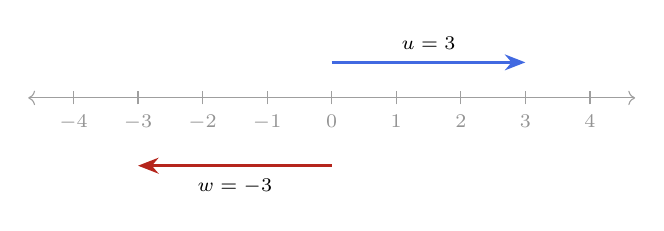
\begin{tikzpicture}[scale=0.82]
  \draw[<->,gray!75,thin] (-4.7,0) -- (4.7,0);
  \foreach \i in {-4,-3,-2,-1,0,1,2,3,4} {
    \draw[gray!75] (\i,-0.1) -- (\i,0.1);
    \node[below,font=\scriptsize,gray!85] at (\i,-0.12) {$\i$};
  }
  \draw[vecarr,RoyalBlue] (0,0.55) -- (3,0.55);
  \node[above,font=\scriptsize] at (1.5,0.6) {$u=3$};
  \draw[vecarr,BrickRed] (0,-1.05) -- (-3,-1.05);
  \node[below,font=\scriptsize] at (-1.5,-1.1) {$w=-3$};
\end{tikzpicture}
\end{center}

%==============================================================================
\section{Notation, and where vectors sit set-theoretically}
%==============================================================================
There are several standard ways to denote a vector symbolically. Using the
letter $v$ purely as an example --- \emph{any} letter may be used:

\begin{center}
\renewcommand{\arraystretch}{1.35}
\begin{tabular}{@{}c l@{}}
\toprule
\textbf{Notation} & \textbf{Reading} \\
\midrule
$\vc{v}$      & boldface --- common in applied and computational writing \\
$\vec{v}$     & arrow overhead --- common in physics and calculus texts \\
$v$           & plain --- common in pure linear algebra, where context suffices \\
\bottomrule
\end{tabular}
\end{center}

\noindent\textbf{In this class we will use a mixture of all three}, and context
will tell you which object you are looking at. Getting comfortable reading all
three is part of the course: you will meet all of them in the reference texts.

\subsection*{The set-theoretic statement}
Until now we have said ``the plane'' in words. Here is its name. To say that
$\vc{v}$ is a two-dimensional vector, we write
\[
  \vc{v}\in\R^{2},
  \qquad\text{where}\qquad
  \R^{2}\;=\;\R\times\R\;=\;\bigl\{(x,y)\;:\;x\in\R,\;y\in\R\bigr\}.
\]
Read aloud: ``$\vc{v}$ is in $\R$-two.'' The superscript $2$ is the dimension of
\S1 --- two coordinates, each free to be any real number, chosen independently.
From here on, $\R^{2}$ replaces ``the plane'' as our standard name for the space
a two-dimensional vector lives in.

\subsection*{The numerical convention for this class}
We write a vector in brackets, listing its coordinates in order:
\[
  \vc{v}=[\,x,\,y\,],
  \qquad\text{for instance}\qquad
  \vc{v}=[\,1,\,2\,].
\]
Order matters: $[1,2]\neq[2,1]$.

\subsection*{Naming a function by what it takes and what it returns}
A steady stream of operations starts in \S7, and we will want a compact way to
record what each one consumes and what it produces --- before saying a word
about how it computes. The standard device is an arrow:
\[
  f : A \to B ,
\]
read ``$f$ from $A$ to $B$'' or ``$f$ maps $A$ to $B$.'' It asserts that $f$
accepts an input drawn from the set $A$ and returns an output lying in the set
$B$. The set $A$ is called the \textbf{domain}, the set $B$ the
\textbf{codomain}, and the statement $f:A\to B$ as a whole is the
\textbf{signature} of $f$.

Notice what a signature deliberately leaves out: the rule. It is a statement
about \emph{types} --- what goes in, what comes out --- and two operations that
compute completely different things may share one.

\smallskip
\noindent\textbf{Two inputs.} Some operations take a pair of arguments rather
than one, and the Cartesian product above is exactly what is needed to say so.
Just as $\R^{2}=\R\times\R$ meant ``ordered pairs of real numbers,''
\[
  \R^{2}\times\R^{2}
  \quad\text{means}\quad
  \text{``ordered pairs of vectors.''}
\]
So an operation swallowing two vectors and returning a vector has signature
$\R^{2}\times\R^{2}\to\R^{2}$, and one swallowing a number and a vector has
signature $\R\times\R^{2}\to\R^{2}$. The number of slots on the left is the
number of arguments.

\smallskip
\noindent\textbf{The placeholder dot.} An operation written with a symbol rather
than a letter needs some way to show its empty argument slots, and the
convention is a centred dot, one per slot. The norm of \S2, for instance, has
signature
\[
  \norm{\,\cdot\,} \;:\; \R^{2}\to\R ,
\]
where the dot marks the place a vector will go. Read it aloud: ``the norm takes
a vector in $\R^{2}$ and returns a real number.'' That is exactly what \S2 said
in words --- one vector in, one number out --- so the notation is not new
content, only a shorthand for something you already know.

It also shows the limits of the device. \S2 also told us the output is never
negative, and the signature cannot say so: its codomain is $\R$, not the
non-negative reals. A signature records the shape of an operation, not its
finer properties.

\lookahead For now we draw every vector with its tail at the origin, so that its
head sits at $(x,y)$. That is a convention, not a restriction: in \S9 we will
see that a vector is really a \emph{displacement}, so the same vector may be
drawn with its tail anywhere in the plane. That fact is what makes the
head-to-tail picture of \S7.1 legitimate.

%==============================================================================
\section{Addition and subtraction}
%==============================================================================
Many operations on vectors await us. Here are the first two.

\begin{defn}[Addition and subtraction in $\R^2$]
Let $\vc{u},\vc{v}\in\R^{2}$ with $\vc{u}=[x_1,y_1]$ and $\vc{v}=[x_2,y_2]$.
Then
\[
  \vc{u}+\vc{v}=[\,x_1+x_2,\;\;y_1+y_2\,],
  \qquad
  \vc{u}-\vc{v}=[\,x_1-x_2,\;\;y_1-y_2\,].
\]
\end{defn}

\noindent Both are \textbf{componentwise}: the first coordinates interact only
with each other, and likewise the second. Nothing mixes across slots.

\smallskip
\noindent Now notice the \emph{shape} of these two operations, exactly as we did
for the norm in \S2. Each one is a \textbf{binary operator}: it consumes
\emph{two} vectors and returns a vector.
\[
  +\;:\;\R^{2}\times\R^{2}\to\R^{2},
  \qquad\qquad
  -\;:\;\R^{2}\times\R^{2}\to\R^{2}.
\]
Read the left-hand side as ``a pair of vectors from $\R^{2}$ goes in.'' Contrast
this with the norm, which was \emph{unary} --- one vector in, one \emph{number}
out. Addition and subtraction are binary, and they never leave $\R^{2}$: two
vectors in, one vector out.

\begin{ex}[Both operations on one pair]
Let $\vc{u}=[2,1]$ and $\vc{v}=[1,3]$. Then
\[
  \vc{u}+\vc{v}=[\,2+1,\;1+3\,]=[\,3,\,4\,],
  \qquad
  \vc{u}-\vc{v}=[\,2-1,\;1-3\,]=[\,1,\,-2\,].
\]
And since we know how to take a norm: $\norm{\vc{u}+\vc{v}}=\sqrt{9+16}=5$ ---
the clean vector from \S2, arrived at by addition.
\end{ex}

%------------------------------------------------------------------------------
\subsection{The parallelogram rule}
%------------------------------------------------------------------------------
Componentwise arithmetic tells you \emph{what} the sum is. Geometry tells you
\emph{where} it is.

\begin{quote}
\textbf{Parallelogram rule.} Place $\vc{u}$ and $\vc{v}$ tail-to-tail at the
origin. They span a parallelogram: the two given arrows are one pair of sides,
and the copies of them drawn from the opposite corners are the other pair. Then
$\vc{u}+\vc{v}$ is the \textbf{diagonal of that parallelogram} running from the
common tail to the far corner.
\end{quote}

\noindent There is a second reading of the same picture, and it is the one to
carry around in your head:

\begin{quote}
\textbf{Head to tail.} Walk along $\vc{u}$. From where you land, walk along
$\vc{v}$. The sum $\vc{u}+\vc{v}$ is the single arrow from where you started to
where you finished.
\end{quote}

\noindent The two readings agree because the far corner of the parallelogram is
reached either way. Notice what the head-to-tail reading quietly does: it draws
$\vc{v}$ with its tail at the head of $\vc{u}$ rather than at the origin. That
is legitimate --- it is the same vector $\vc{v}$, just drawn elsewhere --- and
\S9 is where we make that precise.

In the figure below, the solid arrows are $\vc{u}$, $\vc{v}$ and their sum from
the origin; the dashed arrows are the translated copies that close the
parallelogram. Follow the blue solid arrow and then the green dashed one: you
arrive at $[3,4]$, which is the head of the red diagonal.

\begin{center}
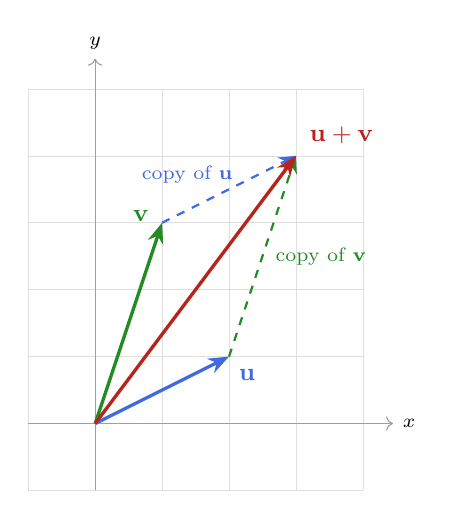
\begin{tikzpicture}[scale=0.85]
  \lattice{-1}{4}{-1}{5}
  \draw[ForestGreen,dashed,thinarr] (2,1) -- (3,4);
  \draw[RoyalBlue,dashed,thinarr]   (1,3) -- (3,4);
  \draw[vecarr,RoyalBlue]   (0,0) -- (2,1);
  \draw[vecarr,ForestGreen] (0,0) -- (1,3);
  \draw[vecarr,BrickRed]    (0,0) -- (3,4);
  \node[below right,font=\small,RoyalBlue]     at (2,0.95)   {$\vc{u}$};
  \node[left,font=\small,ForestGreen]          at (0.95,3.1) {$\vc{v}$};
  \node[right,font=\small,BrickRed]            at (3.06,4.3) {$\vc{u}+\vc{v}$};
  \node[right,font=\scriptsize,ForestGreen]    at (2.55,2.5) {copy of $\vc{v}$};
  \node[left,font=\scriptsize,RoyalBlue]       at (2.2,3.72) {copy of $\vc{u}$};
\end{tikzpicture}
\end{center}

%------------------------------------------------------------------------------
\subsection{The triangle inequality}
%------------------------------------------------------------------------------
Take the head-to-tail picture and ignore the parallelogram: what is left is a
\emph{triangle}. Its three sides have lengths $\norm{\vc{u}}$, $\norm{\vc{v}}$
and $\norm{\vc{u}+\vc{v}}$. And a triangle can never have one side longer than
the other two combined --- walking straight from start to finish cannot be
longer than detouring via a third point.

\begin{quote}
\textbf{Triangle inequality.} For all $\vc{u},\vc{v}\in\R^{2}$,
\[
  \norm{\vc{u}+\vc{v}} \;\le\; \norm{\vc{u}}+\norm{\vc{v}}.
\]
\end{quote}

\noindent Equality holds in exactly one situation: when $\vc{u}$ and $\vc{v}$
point in the \emph{same} direction (or one of them is the zero vector). Then the
``triangle'' has collapsed flat onto a single line, the detour is no detour at
all, and the two sides lie end to end along the third.

\begin{ex}[Strict inequality]
With $\vc{u}=[2,1]$ and $\vc{v}=[1,3]$ from above, $\vc{u}+\vc{v}=[3,4]$ and
\[
  \norm{\vc{u}+\vc{v}}=5,
  \qquad
  \norm{\vc{u}}+\norm{\vc{v}}=\sqrt5+\sqrt{10}\approx 2.236+3.162=5.398 .
\]
Indeed $5<5.398$. The two vectors point in genuinely different directions, so
the detour costs something.
\end{ex}

\begin{ex}[Equality]
Let $\vc{u}=[1,2]$ and $\vc{v}=[2,4]$. Here $\vc{v}$ is just $\vc{u}$ made
twice as long --- same direction --- so we expect equality. And
$\vc{u}+\vc{v}=[3,6]$, so
\[
  \norm{\vc{u}+\vc{v}}=\sqrt{9+36}=\sqrt{45}=3\sqrt5,
  \qquad
  \norm{\vc{u}}+\norm{\vc{v}}=\sqrt5+2\sqrt5=3\sqrt5 .
\]
\end{ex}

\begin{center}
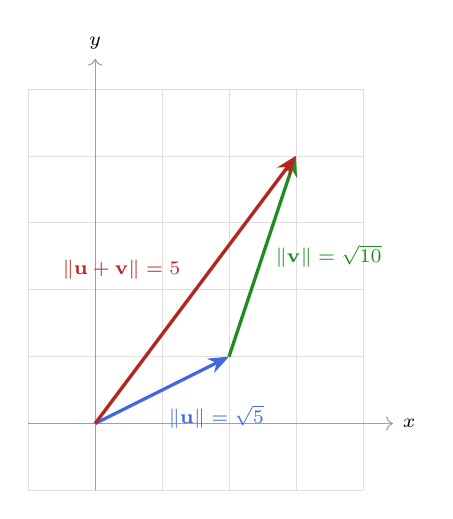
\begin{tikzpicture}[scale=0.85]
  \lattice{-1}{4}{-1}{5}
  \draw[vecarr,RoyalBlue]   (0,0) -- (2,1);
  \draw[vecarr,ForestGreen] (2,1) -- (3,4);
  \draw[vecarr,BrickRed]    (0,0) -- (3,4);
  \node[below right,font=\scriptsize,RoyalBlue]  at (0.95,0.42) {$\norm{\vc{u}}=\sqrt5$};
  \node[right,font=\scriptsize,ForestGreen]      at (2.55,2.5)  {$\norm{\vc{v}}=\sqrt{10}$};
  \node[left,font=\scriptsize,BrickRed]          at (1.42,2.3)  {$\norm{\vc{u}+\vc{v}}=5$};
\end{tikzpicture}
\end{center}

\noindent This inequality is not a curiosity. It is one of the two or three
properties that \emph{define} what it means to be a norm at all, and it is the
reason distances behave the way our intuition expects.

%------------------------------------------------------------------------------
\subsection{Subtraction: the arrow between the heads}
%------------------------------------------------------------------------------
Subtraction has its own picture, and it needs no new machinery.

\begin{quote}
\textbf{Between the heads.} Draw $\vc{u}$ and $\vc{v}$ from the origin. Then
$\vc{u}-\vc{v}$ is the arrow joining the two heads, pointing \emph{from} the
head of $\vc{v}$ \emph{to} the head of $\vc{u}$.
\end{quote}

\noindent It is the displacement that carries you from $\vc{v}$ to $\vc{u}$ ---
which is why differences of vectors are how we will measure how far apart two
vectors are.

\smallskip
\noindent That leaves one thing to get right, and it is the step students most
often reverse: \emph{which way does the arrowhead go?} Here is a rule that never
fails.

\begin{quote}
\textbf{Reading a difference as a journey.} Read $\vc{v}-\vc{u}$ from right to
left: \emph{start at $\vc{u}$, end at $\vc{v}$}. So $\vc{v}-\vc{u}$ points
\emph{at} $\vc{v}$, and $\vc{u}-\vc{v}$ points \emph{at} $\vc{u}$. The arrowhead
always lands on the head of whichever vector is written \emph{first}.
\end{quote}

\noindent And a numerical check, in case the picture ever betrays you: compute
the components and read off their signs. For $\vc{v}-\vc{u}$, the first
coordinate tells you whether the arrow travels right (positive) or left
(negative), and the second tells you up (positive) or down (negative).

\begin{ex}[Both directions on one pair]
Take $\vc{u}=[2,1]$ and $\vc{v}=[1,3]$ again.
\[
  \vc{u}-\vc{v}=[\,1,\,-2\,],
  \qquad
  \vc{v}-\vc{u}=[\,-1,\,2\,].
\]
By the journey rule, $\vc{u}-\vc{v}$ starts at the head of $\vc{v}$, namely
$(1,3)$, and ends at the head of $\vc{u}$, namely $(2,1)$ --- one step right and
two steps down, matching $[\,1,-2\,]$. The other difference,
$\vc{v}-\vc{u}=[-1,2]$, is the same segment travelled backwards: one step left
and two steps up. The two are opposite arrows on the same line.
\end{ex}

\begin{center}
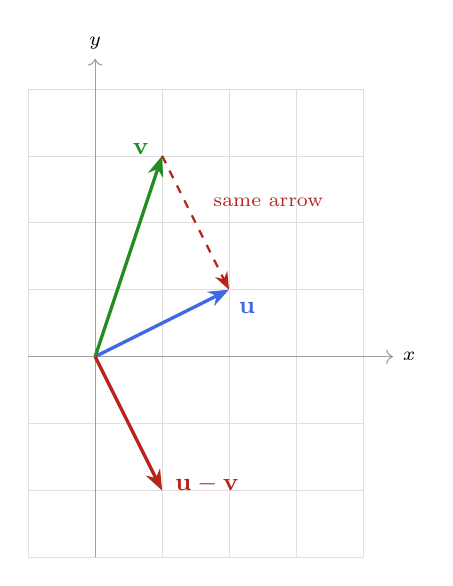
\begin{tikzpicture}[scale=0.85]
  \lattice{-1}{4}{-3}{4}
  \draw[BrickRed,dashed,thinarr] (1,3) -- (2,1);
  \draw[vecarr,RoyalBlue]   (0,0) -- (2,1);
  \draw[vecarr,ForestGreen] (0,0) -- (1,3);
  \draw[vecarr,BrickRed]    (0,0) -- (1,-2);
  \node[below right,font=\small,RoyalBlue] at (2,0.95)     {$\vc{u}$};
  \node[left,font=\small,ForestGreen]      at (0.95,3.1)   {$\vc{v}$};
  \node[right,font=\small,BrickRed]        at (1.05,-1.9)  {$\vc{u}-\vc{v}$};
  \node[right,font=\scriptsize,BrickRed]   at (1.62,2.3)   {same arrow};
\end{tikzpicture}
\end{center}

\noindent The dashed arrow and the solid arrow labelled $\vc{u}-\vc{v}$ are the
\emph{same vector} drawn in two places: same magnitude, same direction,
different tail. \S9 is where that claim gets its definition.

%------------------------------------------------------------------------------
\subsection{Practice: addition and subtraction}
%------------------------------------------------------------------------------
For each pair below: \textbf{(a)} draw $\vc{u}$ and $\vc{v}$ on one set of axes,
tails at the origin, arrowheads marked; \textbf{(b)} compute the indicated sum
or difference componentwise; \textbf{(c)} draw the resulting vector on the same
axes.

\begin{enumerate}[label=\textbf{P\arabic*.},leftmargin=2.8em,itemsep=7pt,
                  topsep=6pt]
  \item $\vc{u}=[3,1]$, \quad $\vc{v}=[1,2]$. \quad Compute $\vc{u}+\vc{v}$.
  \item $\vc{u}=[4,1]$, \quad $\vc{v}=[1,3]$. \quad Compute $\vc{u}-\vc{v}$.
  \item $\vc{u}=[-2,3]$, \quad $\vc{v}=[3,1]$. \quad Compute $\vc{u}+\vc{v}$.
  \item $\vc{u}=[2,-2]$, \quad $\vc{v}=[-3,-1]$. \quad Compute $\vc{u}-\vc{v}$.
\end{enumerate}

\medskip
\noindent\emph{Optional:} compute the norm of each resultant.

\smallskip
\noindent Watch the signs in P4: both inputs have a negative component, so
$2-(-3)=5$ and $-2-(-1)=-1$.

\subsubsection*{Answer key}
\begin{center}
\renewcommand{\arraystretch}{1.3}
\begin{tabular}{@{}c c c c c@{}}
\toprule
\textbf{\#} & $\vc{u}$ & $\vc{v}$ & \textbf{Result} & $\norm{\text{result}}$ \\
\midrule
P1 & $[3,1]$   & $[1,2]$    & $\vc{u}+\vc{v}=[4,3]$   & $5$ \\
P2 & $[4,1]$   & $[1,3]$    & $\vc{u}-\vc{v}=[3,-2]$  & $\sqrt{13}$ \\
P3 & $[-2,3]$  & $[3,1]$    & $\vc{u}+\vc{v}=[1,4]$   & $\sqrt{17}$ \\
P4 & $[2,-2]$  & $[-3,-1]$  & $\vc{u}-\vc{v}=[5,-1]$  & $\sqrt{26}$ \\
\bottomrule
\end{tabular}
\end{center}

%==============================================================================
\section{Scalar multiplication}
%==============================================================================
Addition and subtraction combine a vector with another vector. The next
operation combines a vector with a \emph{scalar} --- one of the plain numbers of
\S4, carrying magnitude but no direction.

\begin{defn}[Scalar multiplication in $\R^2$]
Let $\vc{v}=[\,x,\,y\,]\in\R^{2}$ and let $\alpha\in\R$. Then
\[
  \alpha\vc{v} \;=\; [\,\alpha x,\;\;\alpha y\,].
\]
\end{defn}

\noindent Componentwise again: $\alpha$ multiplies \emph{every} coordinate.

\smallskip
\noindent This operation is binary as well, but its two inputs are of
\emph{different kinds} --- a number and a vector, not two vectors:
\[
  \R\times\R^{2}\to\R^{2}.
\]
A scalar and a vector go in; a vector comes out. That mixed signature is why
$\alpha$ is called a \emph{scalar} in the first place: its job is to set the
scale of the vector.

\begin{ex}[Scaling the running vector]
Let $\vc{v}=[\,1,\,2\,]$, our vector from \S1, with $\norm{\vc{v}}=\sqrt{5}$.
\[
  2\vc{v}=[\,2,\,4\,],
  \qquad
  \tfrac12\vc{v}=[\,\tfrac12,\,1\,],
  \qquad
  -\vc{v}=(-1)\vc{v}=[\,-1,\,-2\,].
\]
Their norms are
\[
  \norm{2\vc{v}}=\sqrt{4+16}=\sqrt{20}=2\sqrt5,
  \qquad
  \norm{\tfrac12\vc{v}}=\sqrt{\tfrac14+1}=\tfrac{\sqrt5}{2},
  \qquad
  \norm{-\vc{v}}=\sqrt{1+4}=\sqrt5 .
\]
So $2\vc{v}$ is twice as long as $\vc{v}$, $\tfrac12\vc{v}$ is half as long, and
$-\vc{v}$ is exactly as long as $\vc{v}$ but points the opposite way.
\end{ex}

\begin{rmk}
Read off the pattern: scaling by $\alpha$ multiplies the magnitude by
$\lvert\alpha\rvert$,
\[
  \norm{\alpha\vc{v}}=\lvert\alpha\rvert\,\norm{\vc{v}},
\]
and the \emph{sign} of $\alpha$ decides the direction --- positive keeps it,
negative reverses it. That is the same sign-carries-direction rule you saw on
the number line in \S5, now acting on a vector in the plane. Taking $\alpha=0$
collapses the vector to $[\,0,\,0\,]$, the \textbf{zero vector}, which has no
direction at all.
\end{rmk}

\Needspace*{13\baselineskip}
\noindent Geometrically, scalar multiplication never turns a vector off its own
line: every multiple of $\vc{v}$ lies on the single straight line through the
origin and the head of $\vc{v}$. Scaling slides the arrowhead along that line
--- stretching it out, pulling it in, or flipping it through the origin --- and
nothing else.

\begin{center}
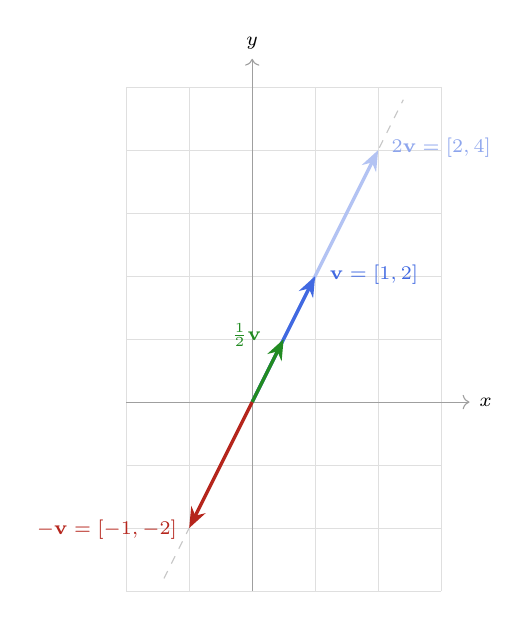
\begin{tikzpicture}[scale=0.8]
  \lattice{-2}{3}{-3}{5}
  % the line through the origin along v -- every multiple of v lands on it
  \draw[gray!45,dashed] (-1.4,-2.8) -- (2.4,4.8);
  \draw[vecarr,RoyalBlue!40] (0,0) -- (2,4);
  \draw[vecarr,RoyalBlue]    (0,0) -- (1,2);
  \draw[vecarr,ForestGreen]  (0,0) -- (0.5,1);
  \draw[vecarr,BrickRed]     (0,0) -- (-1,-2);
  \node[right,font=\scriptsize,RoyalBlue!60] at (2.06,4.04)   {$2\vc{v}=[2,4]$};
  \node[right,font=\scriptsize,RoyalBlue]    at (1.08,2.02)   {$\vc{v}=[1,2]$};
  \node[left,font=\scriptsize,ForestGreen]   at (0.30,1.06)   {$\tfrac12\vc{v}$};
  \node[left,font=\scriptsize,BrickRed]      at (-1.04,-2.02) {$-\vc{v}=[-1,-2]$};
\end{tikzpicture}
\end{center}

%------------------------------------------------------------------------------
\subsection{What scaling does to the picture}
%------------------------------------------------------------------------------
The algebra is one line; the geometry is worth tabulating, because the
\emph{sign} and the \emph{size} of $\alpha$ do two independent jobs. The size
$\lvert\alpha\rvert$ decides the length; the sign decides the direction.

\begin{center}
\renewcommand{\arraystretch}{1.25}
\begin{tabular}{@{}l l l@{}}
\toprule
\textbf{Scalar} & \textbf{Effect on length} & \textbf{Effect on direction} \\
\midrule
$\alpha>1$          & stretched                        & unchanged \\
$\alpha=1$          & unchanged                        & unchanged \\
$0<\alpha<1$        & shrunk                           & unchanged \\
$\alpha=0$          & collapses to the zero vector     & destroyed \\
$-1<\alpha<0$       & shrunk                           & reversed \\
$\alpha=-1$         & unchanged                        & reversed \\
$\alpha<-1$         & stretched                        & reversed \\
\bottomrule
\end{tabular}
\end{center}

\noindent The figure above showed three of these rows on $\vc{v}=[1,2]$:
$\alpha=2$ stretched it, $\alpha=\tfrac12$ shrank it, $\alpha=-1$ reversed it.
The row still missing a picture is the last one --- reversing \emph{and}
stretching at once --- so here it is on a flatter vector, to make the point that
none of this is special to $[1,2]$.

\begin{ex}[Reversing and stretching together]
Let $\vc{w}=[\,2,\,1\,]$, so $\norm{\vc{w}}=\sqrt5$. Then
\[
  2\vc{w}=[\,4,\,2\,],
  \qquad
  -\vc{w}=[\,-2,\,-1\,],
  \qquad
  -2\vc{w}=[\,-4,\,-2\,].
\]
Read the last one geometrically: $\alpha=-2$ is negative, so the arrow turns
around; and $\lvert\alpha\rvert=2$, so it comes out twice as long. All four
arrows lie on one line through the origin --- the two positive multiples on one
side, the two negative multiples on the other.
\end{ex}

\begin{center}
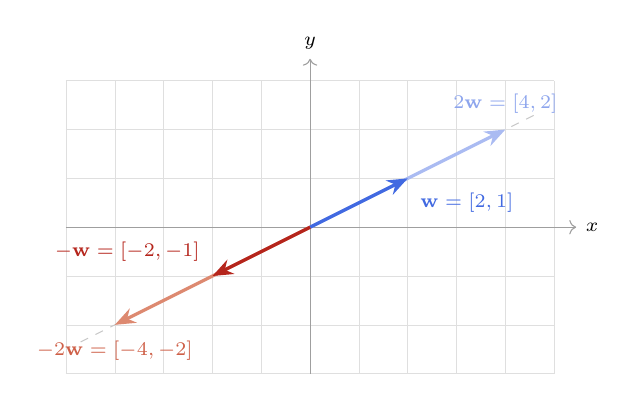
\begin{tikzpicture}[scale=0.62]
  \lattice{-5}{5}{-3}{3}
  \draw[gray!45,dashed] (-4.7,-2.35) -- (4.7,2.35);
  \draw[vecarr,RoyalBlue!45] (0,0) -- (4,2);
  \draw[vecarr,BrickRed!45]  (0,0) -- (-4,-2);
  \draw[vecarr,RoyalBlue]    (0,0) -- (2,1);
  \draw[vecarr,BrickRed]     (0,0) -- (-2,-1);
  \node[above,font=\scriptsize,RoyalBlue!60]   at (4,2.14)      {$2\vc{w}=[4,2]$};
  \node[below right,font=\scriptsize,RoyalBlue] at (2.06,0.9)    {$\vc{w}=[2,1]$};
  \node[above left,font=\scriptsize,BrickRed]  at (-2.06,-0.9)  {$-\vc{w}=[-2,-1]$};
  \node[below,font=\scriptsize,BrickRed!65]    at (-4,-2.14)    {$-2\vc{w}=[-4,-2]$};
\end{tikzpicture}
\end{center}

\noindent The table also runs backwards, which is often how you will use it: if
you can \emph{see} two arrows on a common line through the origin, you can read
off the scalar that relates them without computing anything.

\begin{ex}[Reading the scalar off a picture]
An arrow is drawn on the same line through the origin as $\vc{v}=[1,2]$. It
points the \emph{opposite} way, and it is \emph{three times as long}. Which
multiple of $\vc{v}$ is it?

Opposite direction forces $\alpha<0$; three times as long forces
$\lvert\alpha\rvert=3$. Together, $\alpha=-3$, so the arrow is
\[
  -3\vc{v}=[\,-3,\,-6\,].
\]
Checking against the algebra:
$\norm{-3\vc{v}}=\sqrt{9+36}=\sqrt{45}=3\sqrt5=3\norm{\vc{v}}$, as the picture
promised.
\end{ex}

\begin{ex}[Scaling a physical vector]
Recall from \S4 that velocity is a vector quantity. Let $\vc{v}$ be the velocity
of a car travelling northeast at $30$ mph. Then:
\begin{itemize}[leftmargin=1.4em,itemsep=1pt,topsep=3pt]
  \item $2\vc{v}$ is northeast at $60$ mph --- same heading, twice the speed;
  \item $\tfrac12\vc{v}$ is northeast at $15$ mph --- same heading, half the speed;
  \item $-\vc{v}$ is southwest at $30$ mph --- same speed, reversed heading;
  \item $0\vc{v}$ is the car at rest, with no heading at all.
\end{itemize}
Scaling changes the speed and, if the scalar is negative, the heading --- but it
never turns the car onto a new bearing that is neither the original nor its
exact reverse.
\end{ex}

%------------------------------------------------------------------------------
\subsection{Multiplication by $-1$: mirroring}
%------------------------------------------------------------------------------
The case $\alpha=-1$ deserves a name of its own, because it is the one you will
use constantly.

\begin{quote}
\textbf{Mirroring.} $-\vc{v}=(-1)\vc{v}$ is the \textbf{mirror image of
$\vc{v}$ through the origin}: same line, same length, opposite direction. Every
coordinate flips sign.
\end{quote}

\noindent In the figure above, $\vc{v}=[1,2]$ and $-\vc{v}=[-1,-2]$ sit on
opposite sides of the origin along the same dashed line, at equal distances from
it. The origin is the midpoint of the segment joining their two heads.

\begin{rmk}
Be precise about which mirror. Reflecting \emph{through the origin} --- a point
--- flips \emph{both} coordinates: $[1,2]\mapsto[-1,-2]$. Reflecting
\emph{across an axis} --- a line --- flips only one: across the $x$-axis,
$[1,2]\mapsto[1,-2]$. Multiplication by $-1$ is the first of these, not the
second. Equivalently, it is a half-turn: rotation by $\pi$ about the origin.
\end{rmk}

%------------------------------------------------------------------------------
\subsection{Subtraction revisited: \texorpdfstring{$\vc{u}+(-\vc{v})$}{u + (-v)}}
%------------------------------------------------------------------------------
In \S7.3 we read $\vc{u}-\vc{v}$ off the picture as the arrow between the two
heads. Now that we own the mirror, a second reading opens up --- and it lets us
reuse the parallelogram rule instead of learning a separate recipe.

Subtraction is nothing but addition of the mirror image:
\[
  \vc{u}-\vc{v} \;=\; \vc{u}+(-\vc{v}).
\]
So to subtract geometrically: \textbf{mirror $\vc{v}$ through the origin to get
$-\vc{v}$, then add $\vc{u}$ and $-\vc{v}$ by the parallelogram rule of \S7.1.}
No new geometry at all --- one reflection, then the rule you already have.

\begin{ex}[The same difference, computed two ways]
Take $\vc{u}=[2,1]$ and $\vc{v}=[1,3]$ once more. Mirroring gives
$-\vc{v}=[-1,-3]$, and the parallelogram rule on $\vc{u}$ and $-\vc{v}$ produces
the diagonal
\[
  \vc{u}+(-\vc{v})=[\,2+(-1),\;\;1+(-3)\,]=[\,1,\,-2\,],
\]
which is exactly the $\vc{u}-\vc{v}$ we found in \S7.3. Two different pictures,
one vector.
\end{ex}

\begin{center}
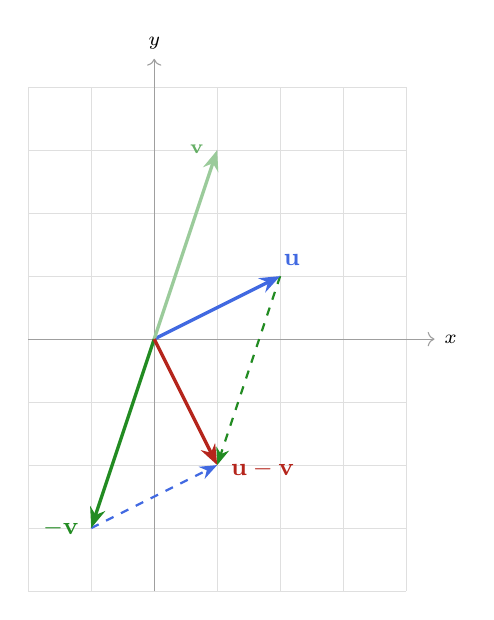
\begin{tikzpicture}[scale=0.8]
  \lattice{-2}{4}{-4}{4}
  % parallelogram on u and -v
  \draw[ForestGreen,dashed,thinarr] (2,1) -- (1,-2);
  \draw[RoyalBlue,dashed,thinarr]   (-1,-3) -- (1,-2);
  \draw[gray!45,dashed] (1,3) -- (-1,-3);
  \draw[vecarr,RoyalBlue]        (0,0) -- (2,1);
  \draw[vecarr,ForestGreen!45]   (0,0) -- (1,3);
  \draw[vecarr,ForestGreen]      (0,0) -- (-1,-3);
  \draw[vecarr,BrickRed]         (0,0) -- (1,-2);
  \node[above right,font=\small,RoyalBlue]      at (1.9,1.02)   {$\vc{u}$};
  \node[left,font=\scriptsize,ForestGreen!70]   at (0.94,3.02)  {$\vc{v}$};
  \node[left,font=\small,ForestGreen]           at (-1.04,-3.0) {$-\vc{v}$};
  \node[right,font=\small,BrickRed]             at (1.06,-2.06) {$\vc{u}-\vc{v}$};
\end{tikzpicture}
\end{center}

\noindent The faint green arrow is the original $\vc{v}$; the solid green one is
its mirror image $-\vc{v}$, and the faint dashed line through the origin shows
that the two really do lie on a common line. The red diagonal of the
parallelogram spanned by $\vc{u}$ and $-\vc{v}$ is $\vc{u}-\vc{v}$.

%==============================================================================
\section{When are two vectors equal?}
%==============================================================================
We have twice now drawn ``the same vector'' in two different places and asked
you to believe it. Time to define it.

\begin{defn}[Equality of vectors]
Two vectors are \textbf{equal} when they have the same magnitude \emph{and} the
same direction. In components, for $\vc{u}=[u_1,u_2]$ and $\vc{v}=[v_1,v_2]$,
\[
  \vc{u}=\vc{v}
  \qquad\Longleftrightarrow\qquad
  u_1=v_1 \;\;\text{and}\;\; u_2=v_2 .
\]
\end{defn}

\noindent Notice what the definition does \emph{not} mention: where the arrow
is. A vector is a magnitude together with a direction --- a
\emph{displacement} --- and a displacement does not care where you start it.

\subsection*{Components from any tail: head minus tail}
So how do you read the components off an arrow that does not start at the
origin? Subtract.

\begin{quote}
An arrow with tail $A=(a_1,a_2)$ and head $B=(b_1,b_2)$ is the vector
\[
  [\,b_1-a_1,\;\;b_2-a_2\,]
  \qquad\text{---}\qquad
  \textbf{head minus tail}.
\]
\end{quote}

\noindent This is not a new rule; it is the subtraction of \S7.3 seen from the
other side. Two arrows are the same vector precisely when their
head-minus-tail differences agree, no matter how far apart the arrows are
drawn. Every vector therefore has infinitely many drawings, called
\emph{representatives}, and exactly one of them has its tail at the origin ---
that one is said to be in \textbf{standard position}, and it is the drawing we
have been defaulting to since \S1.

\begin{ex}[Three drawings, one vector]
Each of these arrows is the vector $[\,2,\,1\,]$:
\begin{enumerate}[label=(\roman*),leftmargin=2.4em,itemsep=2pt,topsep=3pt]
  \item tail $(0,0)$, head $(2,1)$: \quad $[\,2-0,\;1-0\,]=[\,2,\,1\,]$;
  \item tail $(1,3)$, head $(3,4)$: \quad $[\,3-1,\;4-3\,]=[\,2,\,1\,]$;
  \item tail $(-3,-1)$, head $(-1,0)$: \quad $[\,-1-(-3),\;0-(-1)\,]=[\,2,\,1\,]$.
\end{enumerate}
They sit in three different places on the page. They are the same vector: each
one says ``two steps right, one step up.''
\end{ex}

\begin{ex}[Same magnitude is not enough]
$[\,1,\,2\,]$ and $[\,2,\,1\,]$ both have norm $\sqrt5$, so they are equally
long --- but the first climbs steeply and the second runs flat. Different
directions, so they are \emph{different vectors}.
\end{ex}

\begin{ex}[Same direction is not enough either]
$[\,1,\,2\,]$ and $[\,2,\,4\,]$ point exactly the same way --- the second is
$2$ times the first, so by \S8 they lie on one line through the origin --- but
their norms are $\sqrt5$ and $2\sqrt5$. Different magnitudes, so again
\emph{different vectors}.
\end{ex}

\begin{ex}[Mirrors are not equal]
$[\,1,\,2\,]$ and $[\,-1,\,-2\,]$ have the same norm $\sqrt5$ and lie on the
same line, but they point opposite ways. By \S8.2 the second is the mirror image
of the first, and a mirror image is a \emph{different vector} --- unless the
vector is $[\,0,\,0\,]$, which is its own mirror.
\end{ex}

\noindent Equality needs \emph{both} attributes to match. The last three
examples fail on exactly one apiece.

\begin{warn}
An arrow drawn near the top of the page and an arrow drawn near the bottom
\emph{look} like two different objects, and it is tempting to treat them as two
different vectors. They are not, so long as head minus tail comes out the same
for both. Conversely, two arrows can start at the very same point and still be
different vectors. Position on the page is not part of the data; magnitude and
direction are.
\end{warn}

\begin{center}
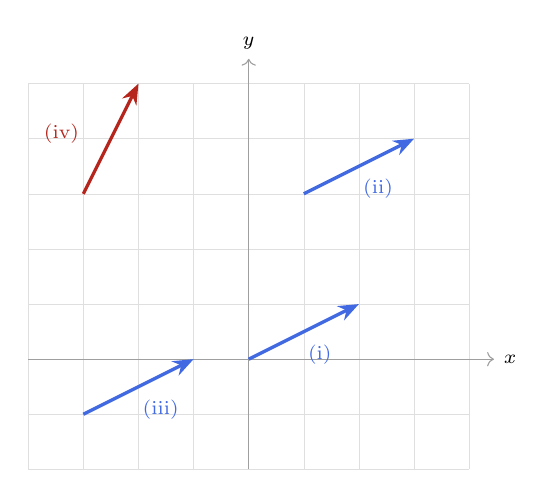
\begin{tikzpicture}[scale=0.7]
  \lattice{-4}{4}{-2}{5}
  \draw[vecarr,RoyalBlue] (0,0)   -- (2,1);
  \draw[vecarr,RoyalBlue] (1,3)   -- (3,4);
  \draw[vecarr,RoyalBlue] (-3,-1) -- (-1,0);
  \draw[vecarr,BrickRed]  (-3,3)  -- (-2,5);
  \node[below right,font=\scriptsize,RoyalBlue] at (0.9,0.44)  {(i)};
  \node[below right,font=\scriptsize,RoyalBlue] at (1.9,3.44)  {(ii)};
  \node[below right,font=\scriptsize,RoyalBlue] at (-2.1,-0.56){(iii)};
  \node[left,font=\scriptsize,BrickRed]         at (-2.9,4.1)  {(iv)};
\end{tikzpicture}
\end{center}

\noindent Arrows (i), (ii) and (iii) are the three representatives of
$[\,2,\,1\,]$ from the example above: parallel, equally long, all pointing the
same way, and therefore \emph{one and the same vector}. Arrow (iv) is
$[\,1,\,2\,]$; it has the same length $\sqrt5$ as the others but a different
direction, so it is a different vector.

\end{document}
